\documentclass{beamer}
\mode<presentation>{
  \usetheme{Boadilla}
  \usefonttheme[onlylarge]{structurebold}
  \usefonttheme[stillsansseriflarge]{serif}
  \setbeamerfont*{frametitle}{size=\normalsize,series=\bfseries}
  % \setbeamertemplate{navigation symbols}{}
  \setbeamercovered{transparent}
}
\usepackage[english]{babel}
\usepackage[latin1]{inputenc}
\usepackage{times}
\usepackage[T1]{fontenc}
\usepackage{amsmath}
\usepackage{amssymb}
\usepackage{esint}
\usepackage{hyperref}
\usepackage{tikz}
\usepackage{xkeyval}
\usepackage{xargs}
\usepackage{verbatim}
\usepackage{listings}
\usepackage{multimedia}
\usetikzlibrary{
  arrows,
  calc,
  decorations.pathmorphing,
  decorations.pathreplacing,
  decorations.markings,
  fadings,
  positioning,
  shapes
}

\pgfdeclareradialshading{glow}{\pgfpoint{0cm}{0cm}}{
  color(0mm)=(white);
  color(3mm)=(white);
  color(7mm)=(black);
  color(10mm)=(black)
}

\begin{tikzfadingfrompicture}[name=glow fading]
  \shade [shading=glow] (0,0) circle (1);
\end{tikzfadingfrompicture}

\mode<handout>{
  \usepackage{pgfpages}
  \pgfpagesuselayout{4 on 1}[a4paper,landscape,border shrink=5mm]
  \setbeamercolor{background canvas}{bg=black!10}
}

\newcommand\pgfmathsinandcos[3]{%
  \pgfmathsetmacro#1{sin(#3)}%
  \pgfmathsetmacro#2{cos(#3)}%
}
\newcommand\LongitudePlane[3][current plane]{%
  \pgfmathsinandcos\sinEl\cosEl{#2} % elevation
  \pgfmathsinandcos\sint\cost{#3} % azimuth
  \tikzset{#1/.estyle={cm={\cost,\sint*\sinEl,0,\cosEl,(0,0)}}}
}
\newcommand\LatitudePlane[3][current plane]{%
  \pgfmathsinandcos\sinEl\cosEl{#2} % elevation
  \pgfmathsinandcos\sint\cost{#3} % latitude
  \pgfmathsetmacro\yshift{\cosEl*\sint}
  \tikzset{#1/.estyle={cm={\cost,0,0,\cost*\sinEl,(0,\yshift)}}} %
}
\newcommand\DrawLongitudeCircle[2][1]{
  \LongitudePlane{\angEl}{#2}
  \tikzset{current plane/.prefix style={scale=#1}}
  % angle of "visibility"
  \pgfmathsetmacro\angVis{atan(sin(#2)*cos(\angEl)/sin(\angEl))} %
  \draw[current plane] (\angVis:1) arc (\angVis:\angVis+180:1);
  \draw[current plane,dashed] (\angVis-180:1) arc (\angVis-180:\angVis:1);
}
\newcommand\DrawLatitudeCircleArrow[2][1]{
  \LatitudePlane{\angEl}{#2}
  \tikzset{current plane/.prefix style={scale=#1}}
  \pgfmathsetmacro\sinVis{sin(#2)/cos(#2)*sin(\angEl)/cos(\angEl)}
  % angle of "visibility"
  \pgfmathsetmacro\angVis{asin(min(1,max(\sinVis,-1)))}
  \draw[current plane,decoration={markings, mark=at position 0.6 with {\arrow{<}}},postaction={decorate},line width=.6mm] (\angVis:1) arc (\angVis:-\angVis-180:1);
  \draw[current plane,dashed,line width=.6mm] (180-\angVis:1) arc (180-\angVis:\angVis:1);
}
\newcommand\DrawLatitudeCircle[2][1]{
  \LatitudePlane{\angEl}{#2}
  \tikzset{current plane/.prefix style={scale=#1}}
  \pgfmathsetmacro\sinVis{sin(#2)/cos(#2)*sin(\angEl)/cos(\angEl)}
  % angle of "visibility"
  \pgfmathsetmacro\angVis{asin(min(1,max(\sinVis,-1)))}
  \draw[current plane] (\angVis:1) arc (\angVis:-\angVis-180:1);
  \draw[current plane,dashed] (180-\angVis:1) arc (180-\angVis:\angVis:1);
}
\newcommand\coil[1]{
  {\rh * cos(\t * pi r)}, {\apart * (2 * #1 + \t) + \rv * sin(\t * pi r)}
}
\makeatletter
\define@key{DrawFromCenter}{style}[{->}]{
  \tikzset{DrawFromCenterPlane/.style={#1}}
}
\define@key{DrawFromCenter}{r}[1]{
  \def\@R{#1}
}
\define@key{DrawFromCenter}{center}[(0, 0)]{
  \def\@Center{#1}
}
\define@key{DrawFromCenter}{theta}[0]{
  \def\@Theta{#1}
}
\define@key{DrawFromCenter}{phi}[0]{
  \def\@Phi{#1}
}
\presetkeys{DrawFromCenter}{style, r, center, theta, phi}{}
\newcommand*\DrawFromCenter[1][]{
  \setkeys{DrawFromCenter}{#1}{
    \pgfmathsinandcos\sint\cost{\@Theta}
    \pgfmathsinandcos\sinp\cosp{\@Phi}
    \pgfmathsinandcos\sinA\cosA{\angEl}
    \pgfmathsetmacro\DX{\@R*\cost*\cosp}
    \pgfmathsetmacro\DY{\@R*(\cost*\sinp*\sinA+\sint*\cosA)}
    \draw[DrawFromCenterPlane] \@Center -- ++(\DX, \DY);
  }
}
\newcommand*\DrawFromCenterText[2][]{
  \setkeys{DrawFromCenter}{#1}{
    \pgfmathsinandcos\sint\cost{\@Theta}
    \pgfmathsinandcos\sinp\cosp{\@Phi}
    \pgfmathsinandcos\sinA\cosA{\angEl}
    \pgfmathsetmacro\DX{\@R*\cost*\cosp}
    \pgfmathsetmacro\DY{\@R*(\cost*\sinp*\sinA+\sint*\cosA)}
    \draw[DrawFromCenterPlane] \@Center -- ++(\DX, \DY) node {#2};
  }
}
\makeatother

% not mandatory, but I though it was better to set it blank
\setbeamertemplate{headline}{}
\def\beamer@entrycode{\vspace{-\headheight}}

\tikzstyle{snakearrow} = [decorate, decoration={pre length=0.2cm,
  post length=0.2cm, snake, amplitude=.4mm,
  segment length=2mm},thick, ->]

%% document-wide tikz options and styles

\tikzset{%
  % >=latex, % option for nice arrows
  inner sep=0pt,%
  outer sep=2pt,%
  mark coordinate/.style={inner sep=0pt,outer sep=0pt,minimum size=3pt,
    fill=black,circle}%
}
\tikzset{
  % Define standard arrow tip
  >=stealth',
  % Define style for boxes
  punkt/.style={
    rectangle,
    rounded corners,
    draw=black, very thick,
    text width=8em,
    minimum height=2.5em,
    text centered},
}
\makeatletter
\newbox\@backgroundblock
\newenvironment{backgroundblock}[2]{%
  \global\setbox\@backgroundblock=\vbox\bgroup%
  \unvbox\@backgroundblock%
  \vbox to0pt\bgroup\vskip#2\hbox to0pt\bgroup\hskip#1\relax%
}{\egroup\egroup\egroup}
\addtobeamertemplate{background}{\box\@backgroundblock}{}
\makeatother

\def\theauthor{Yichao Yu}
\def\theinstitute{Ni Group/Harvard}
\title{Trapping and imaging of single atom in the present of light shift}
\author{\theauthor}
\institute{\theinstitute}
\date{May 5, 2015}
\makeatletter
\def\thedate{\@date}
\makeatother

\begin{document}

% As mentioned in the previous talk, the goal of the experiment is to
% make dipolar molecules using trapped single atoms.

% Talk about some techniques we use in one of the important step:
% (discovered and solved problems)
% -    Trap single atom with tweezer out of laser cooled gas.
% <figure 1>
% How hard can this be =p

\begin{frame}[t]{}
  \begin{center}
    \usebeamerfont{title}{\usebeamercolor[fg]{title}{\inserttitle\par}}
  \end{center}
  \begin{columns}[t]
    \column{8cm}
    {}
    % Somehow the author and date etc moves to the bottom of the
    % page if this is removed.....
    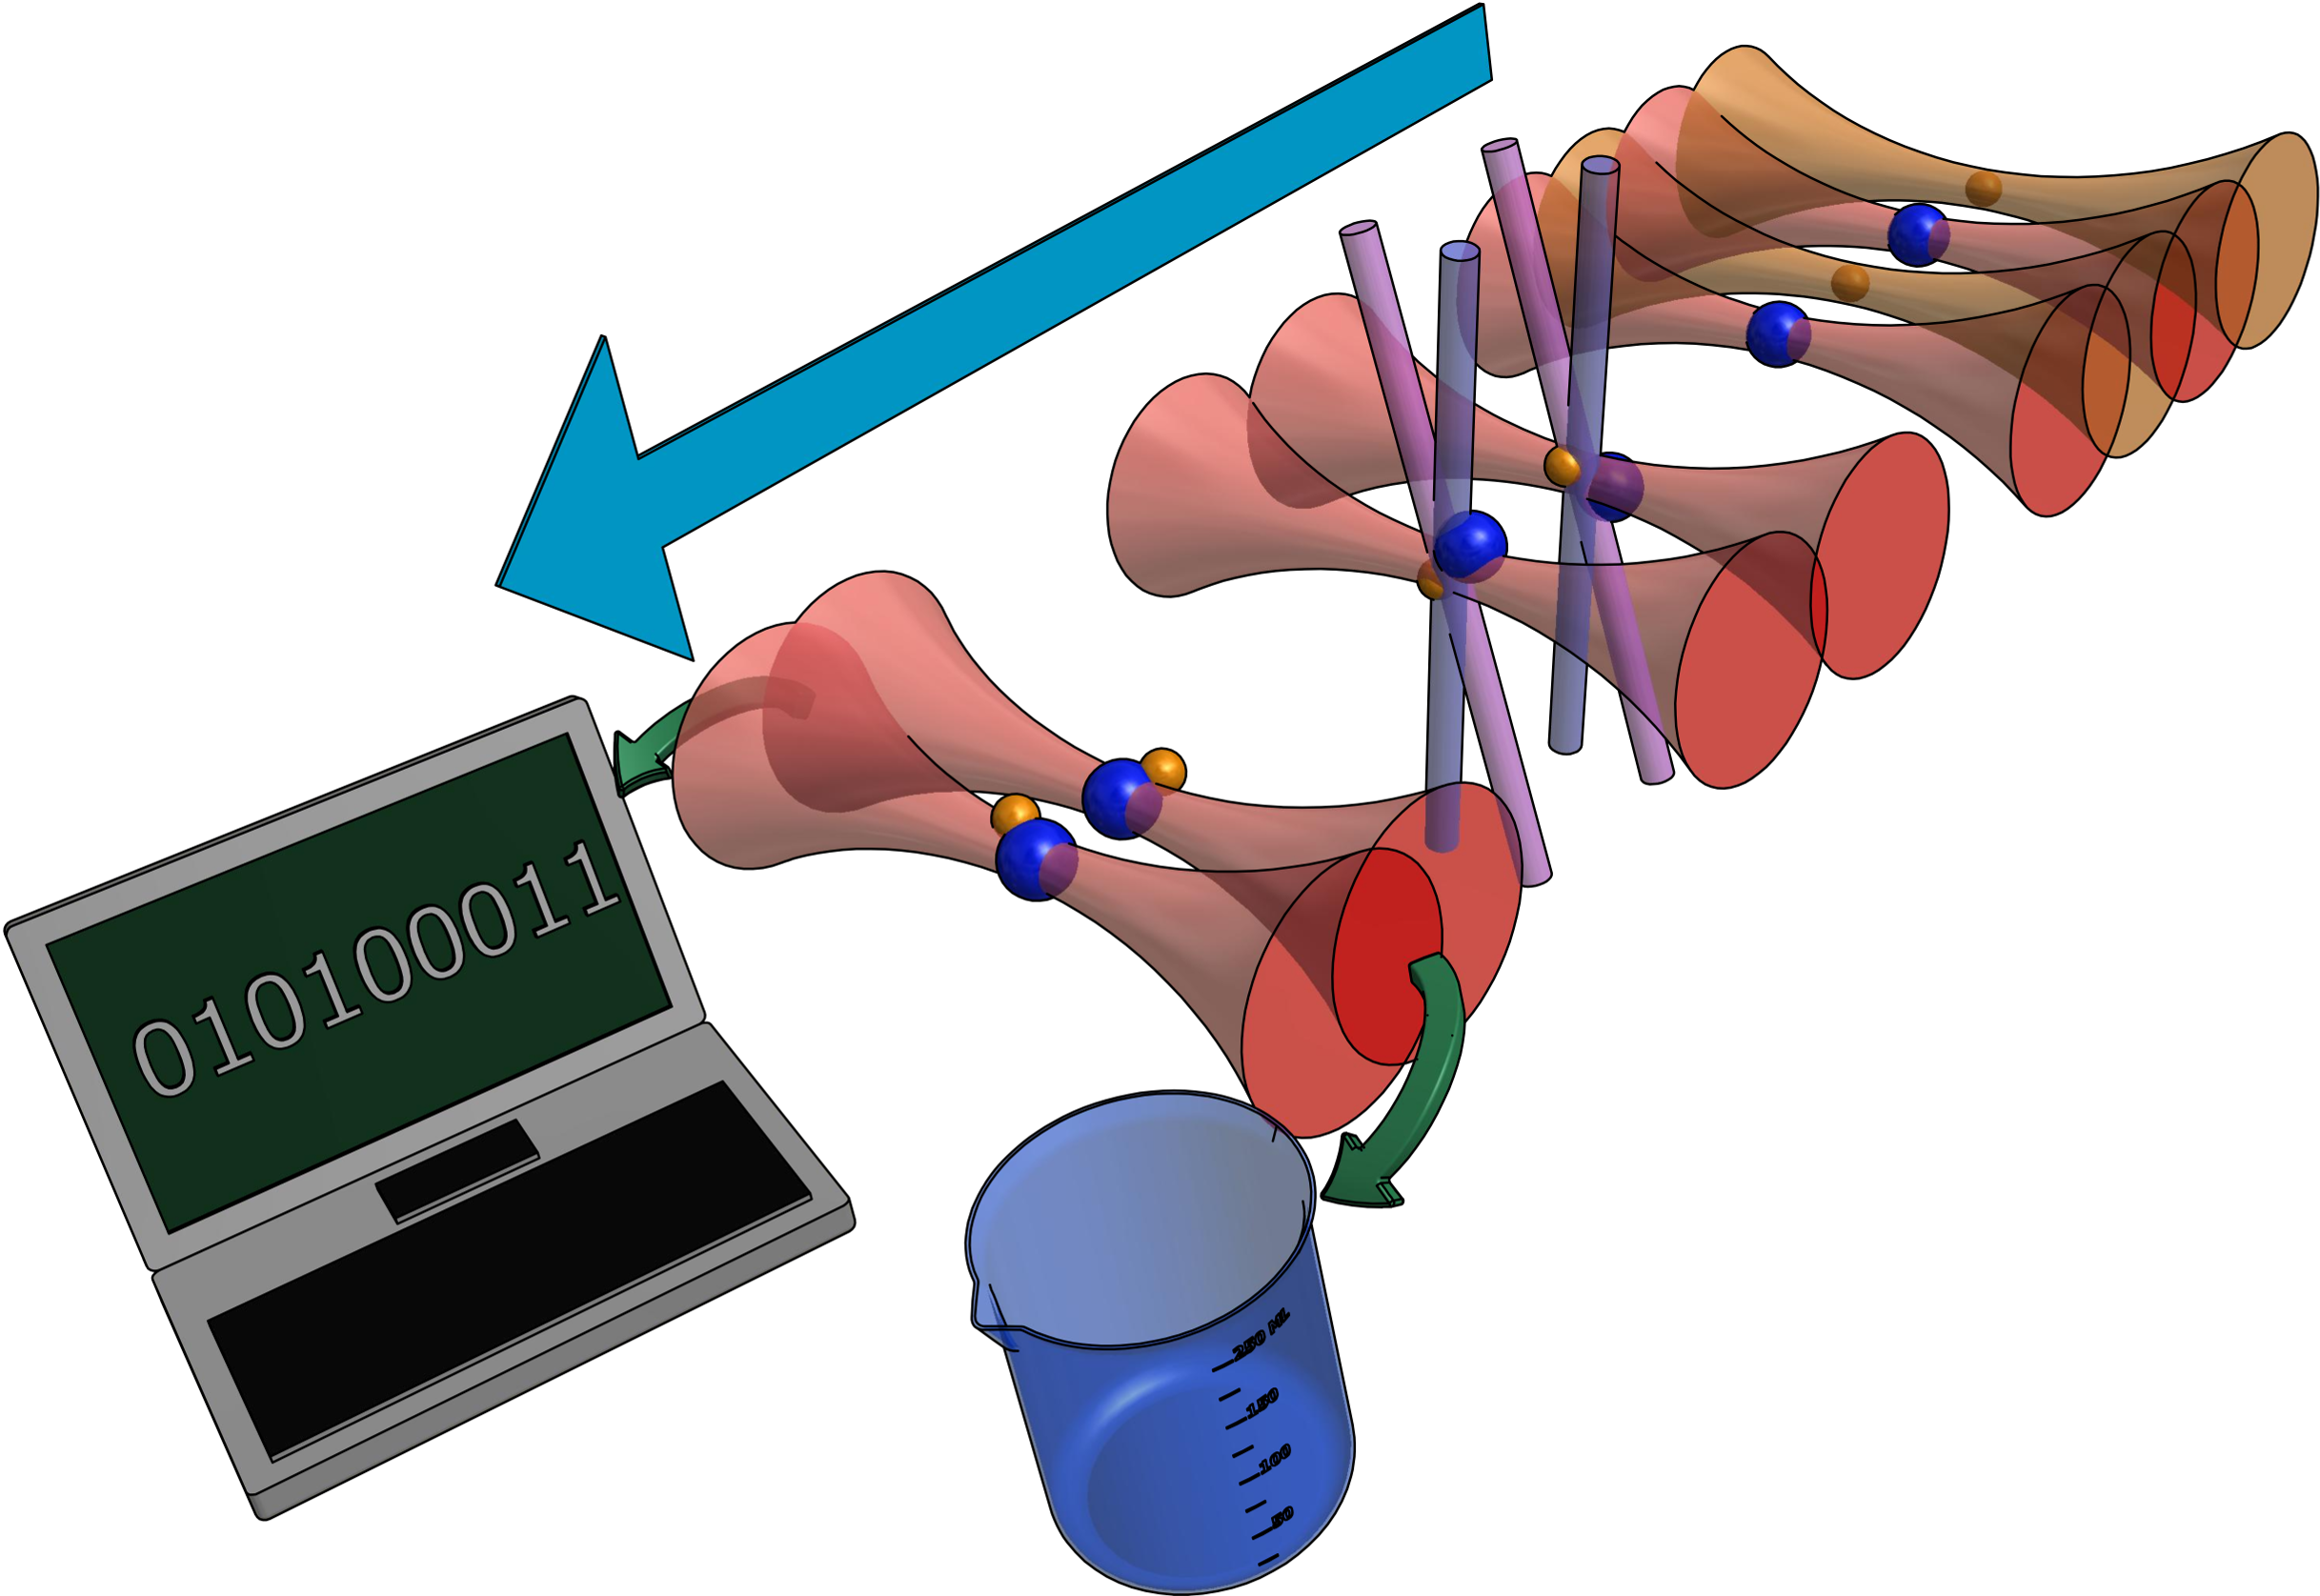
\includegraphics[width=8cm]{overall_full_min.png}
    \column{4cm}
    \begin{center}
      \usebeamercolor[fg]{title}{
        {\large{\theauthor}}\\
        {\small{\thedate}}\\
        {\small{\theinstitute}}}
    \end{center}
  \end{columns}
\end{frame}

% Done in Rb by ....
% - Load MOT
% - Trap with tweezer
% - Image
% Objective + EMCCD
% <figure 2> <animated>
% Didn't take so long for Cs (picture)
% <figure 3> Image, histogram

\begin{frame}
  \begin{columns}[t]
    \column{5cm}
    \begin{block}{\only<1>{Single atom loading}
        \only<2->{Procedure}}
      \begin{itemize}
      \item<1-> Similar to\\
        Ref1\\
        Ref2
      \item<2-> MOT Loading
      \item<3-> Trapping
      \item<4-> Imaging
      \item<5-> Works for Cs
      \end{itemize}
    \end{block}
    \column{7cm}
    \begin{center}
      \begin{tikzpicture}
        \visible<2-3>{
          \shade[shading=radial,inner color=orange] (0,0) circle (1);
        }
        \visible<3-4>{
          \shade[shading=radial,rotate=90,yscale=1,fill opacity=0.8,
          inner color=red]
          plot[draw,samples=200,domain=-3:3] function {sqrt(0.0025 + x**2 / 10)}
          -- plot[draw,samples=200,domain=3:-3] function {-sqrt(0.0025 + x**2 / 10)};
          \fill [blue,path fading=glow fading] (0,0) circle (0.08);
          % the fading effect
        }
        \visible<5> {
          % TODO replace with a better one
          \path (0,0) node[above]
          {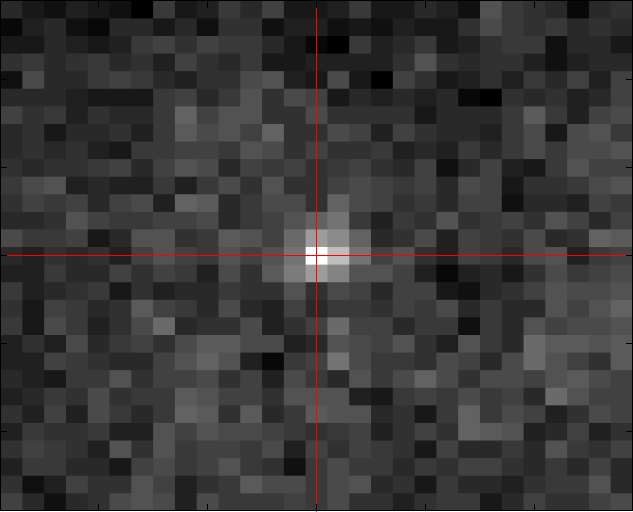
\includegraphics[width=4cm]{Cs_single_atom.png}};
          % TODO add histogram
          \path (0,0) node[below] {Add Histogram};
        }
      \end{tikzpicture}
    \end{center}
  \end{columns}
\end{frame}

% Doesn't work for Na
% For Na we saw (blank picture)
% We believe the issue is Light shift

% \beta parameter, due to multiple levels. 1 = magic

% Problems caused by this:
% 1. Loading
% -    Inefficient cooling
% 2. Imaging

\begin{frame}
\end{frame}

\begin{frame}
\end{frame}

% Solution:
% * Switching
% * Fast enough (comparing to trap frequency)
% * Slow enough (comparing to excited stated lifetime)

% Result
% * Single Na atom

\begin{frame}[t]
  % \vspace{-0.8cm}
  % \begin{columns}[t]
  %   \column{4cm}
  %   \begin{center}
  %     Prof. Kang-Kuen\\
  %     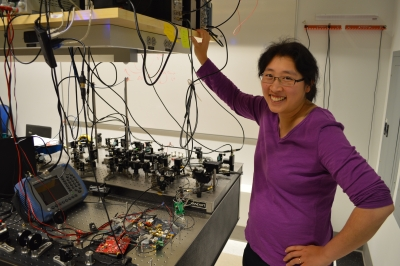
\includegraphics[width=3.5cm]{KangKuen.jpg}\\
  %     Nick (NaCs)\\
  %     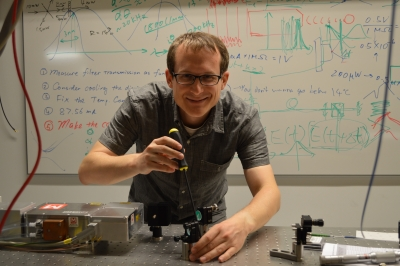
\includegraphics[width=3.5cm]{Nick.jpg}\\
  %     Lee (NaCs)\\
  %     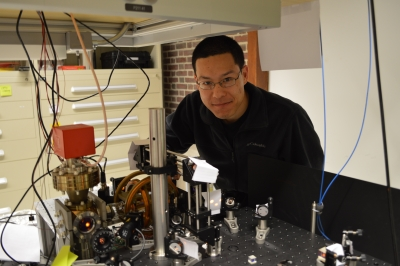
\includegraphics[width=3.5cm]{Lee.jpg}
  %   \end{center}
  %   \column{4cm}
  %   \begin{center}
  %     Yu (KRb)\\
  %     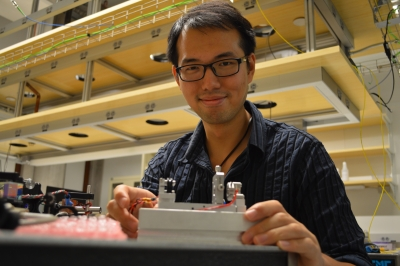
\includegraphics[width=3.5cm]{Yu.jpg}\\
  %     Hyungmok (KRb)\\
  %     \includegraphics[width=3.5cm]{Jim1.jpg}
  %   \end{center}
  %   \column{4cm}
  %   \begin{center}
  %     Saahil (Undergrad.)\\
  %     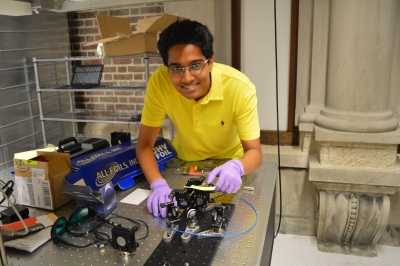
\includegraphics[width=3.5cm]{Saahil.jpg}\\
  %     Will (Undergrad.)\\
  %     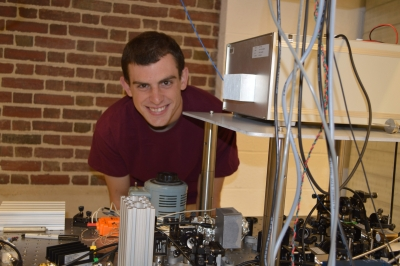
\includegraphics[width=3.5cm]{Will.jpg}
  %   \end{center}
  % \end{columns}
\end{frame}

\begin{frame}
\end{frame}

\begin{frame}
  % \begin{center}
  %   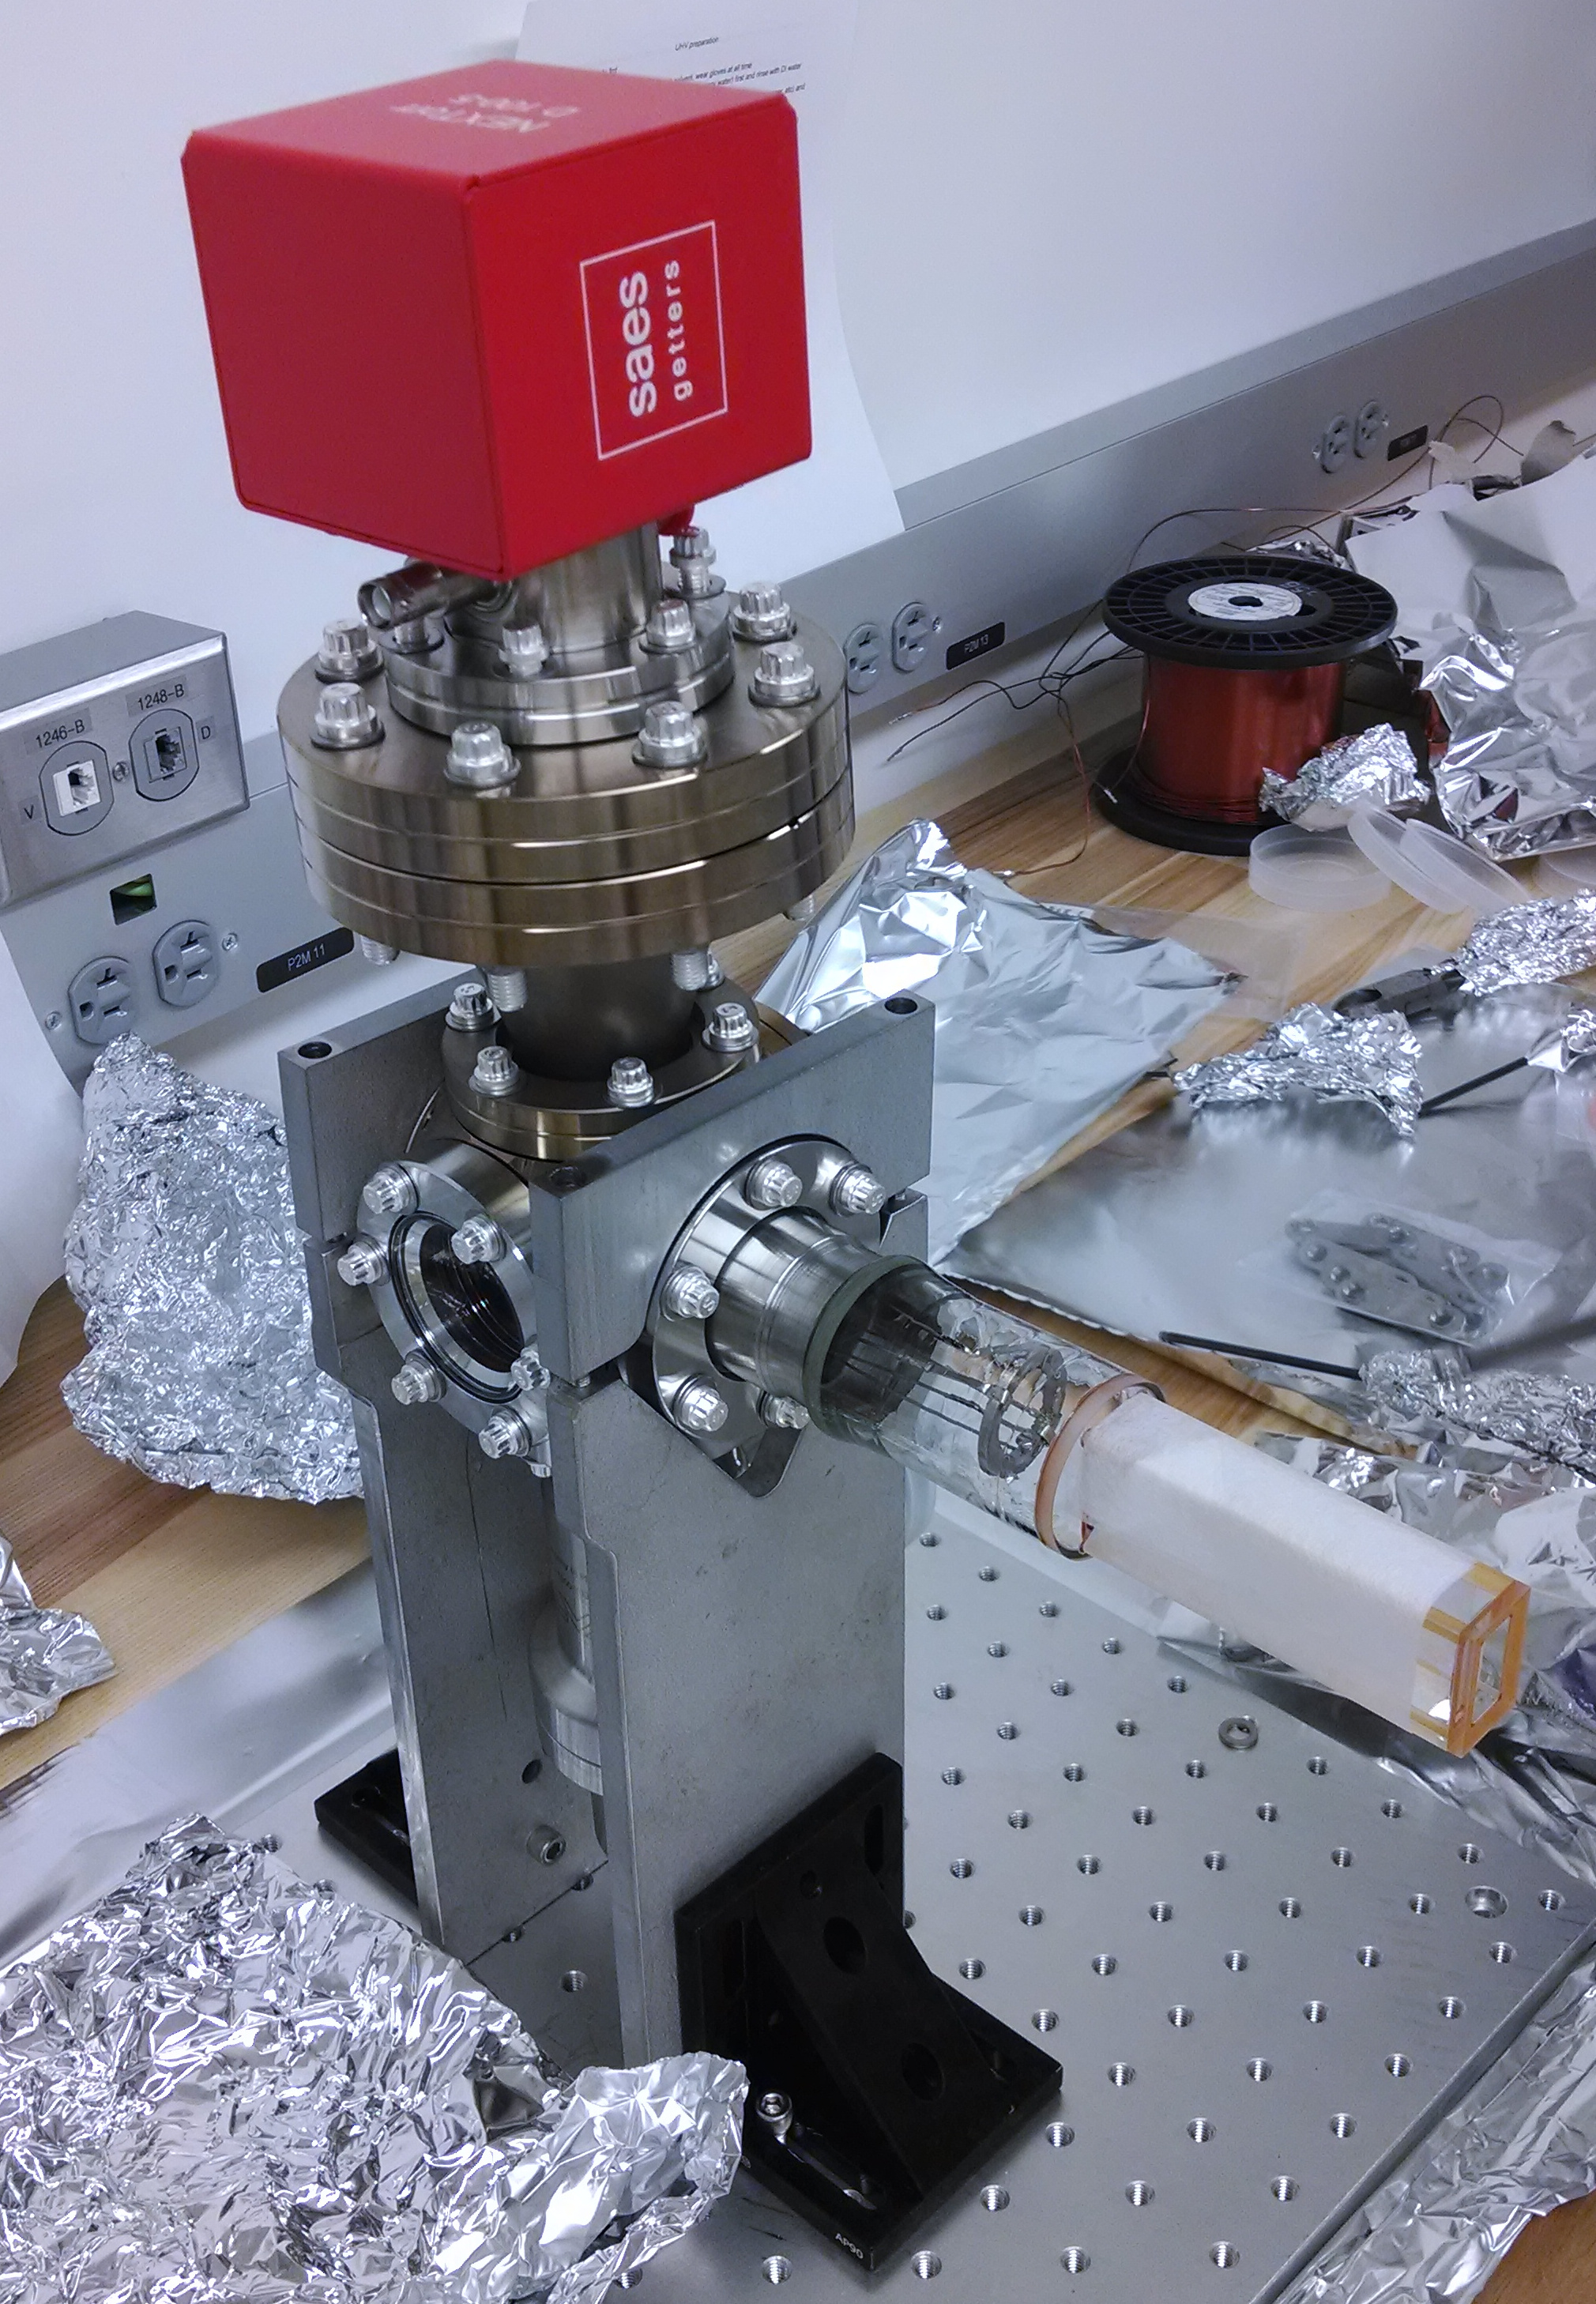
\includegraphics[height=8cm]{chamber.jpg}
  % \end{center}
\end{frame}

\end{document}
